\documentclass[border=10pt]{standalone}
\usepackage[svgnames]{xcolor}
\usepackage{amsmath}
\usepackage{pgfplots}
\pgfplotsset{compat=newest}
\usepackage[sfdefault]{FiraSans}
\usepackage{FiraMono}
\renewcommand*\familydefault{\sfdefault}
\begin{document}
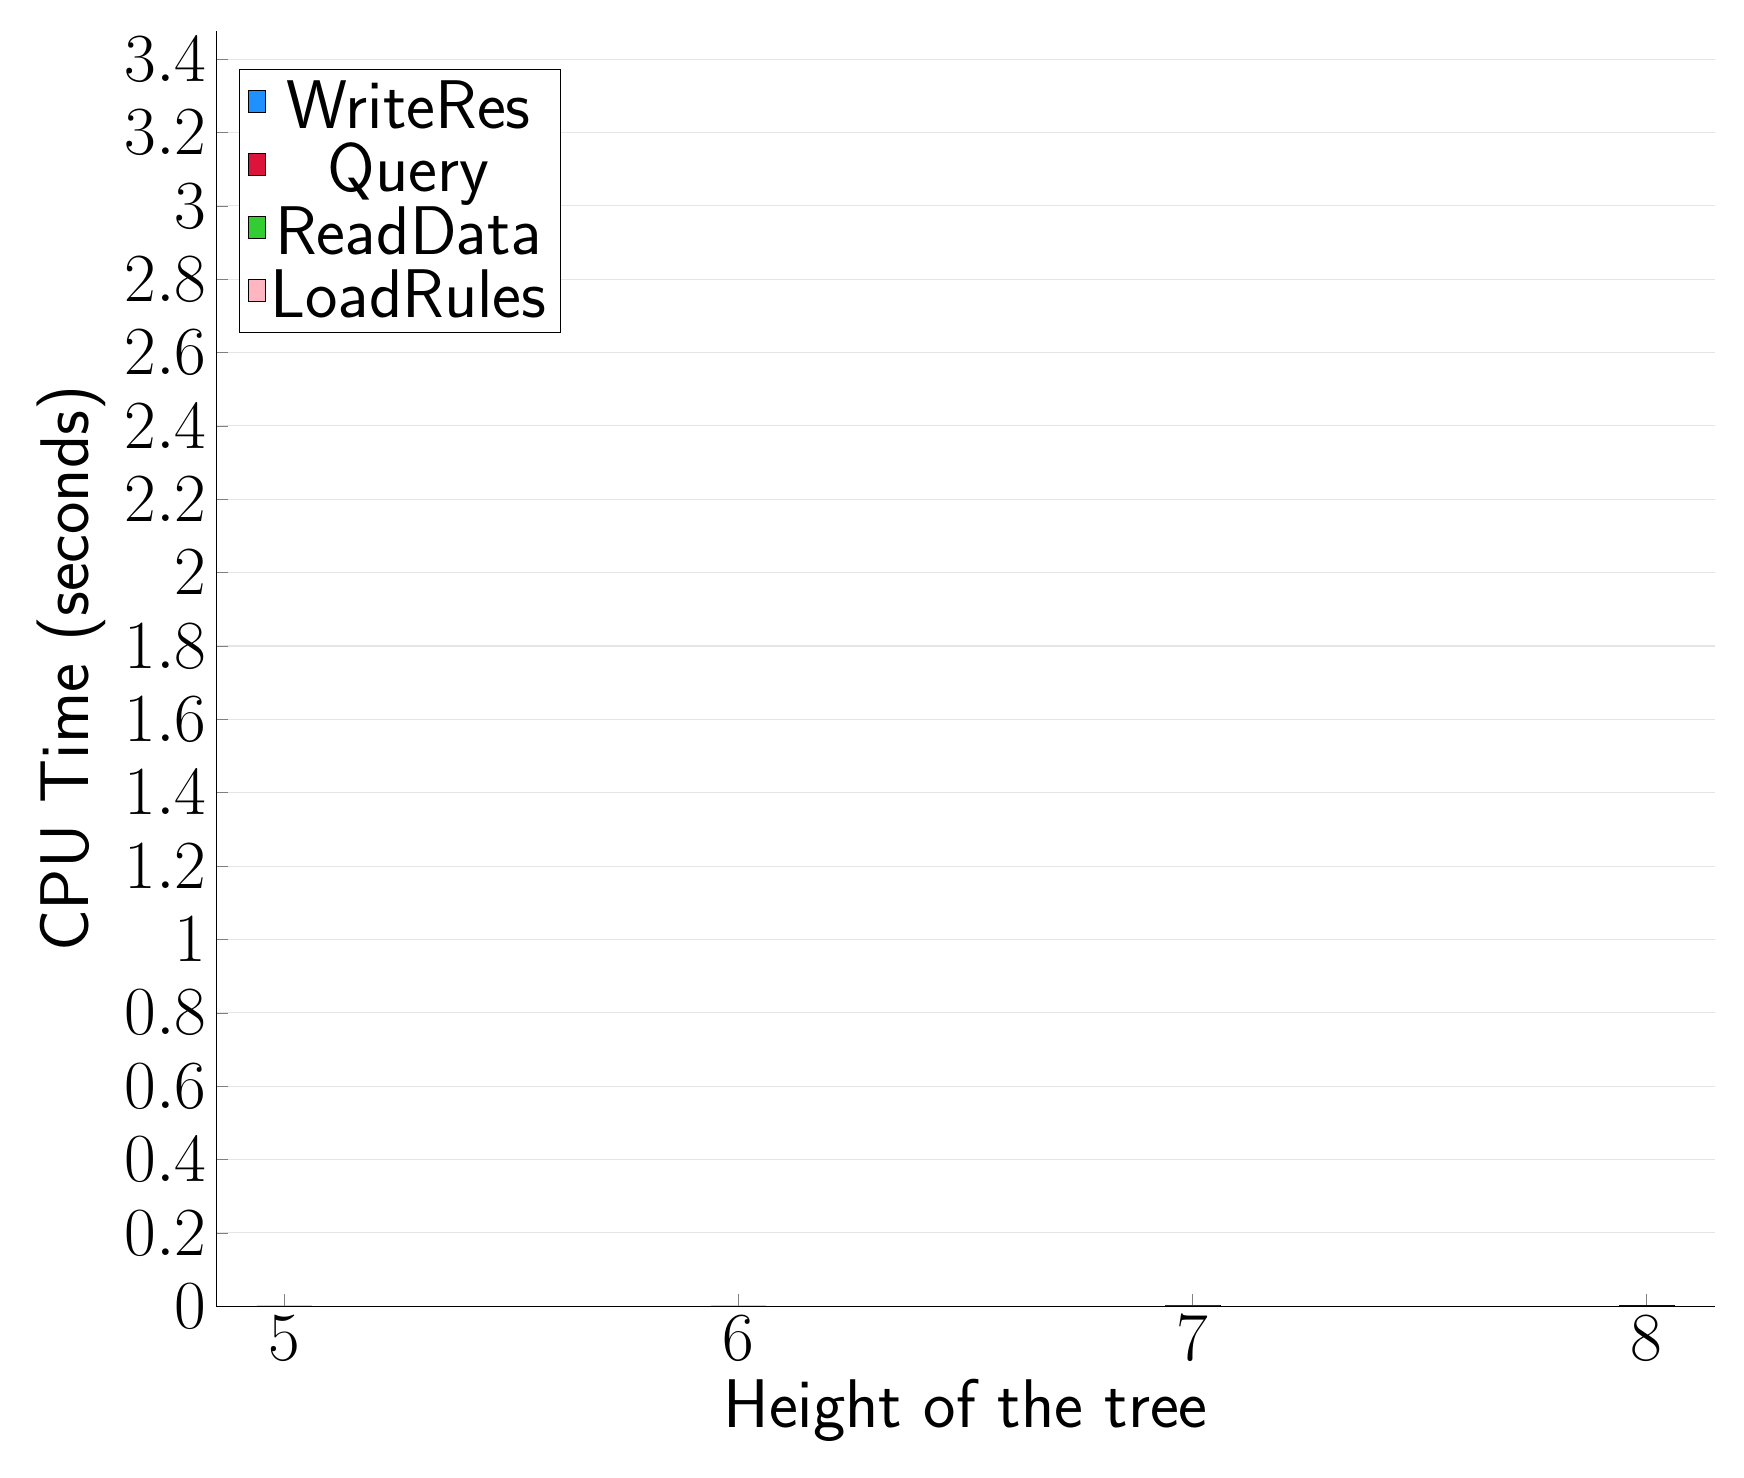
\begin{tikzpicture}
\begin{axis}[
   ybar stacked,
   width=1.7\textwidth,
   bar width=0.7cm,
   ymajorgrids, tick align=inside,
   major grid style={draw=gray!20},
   xtick=data,
   ymin=0, ymax=3.477,
   axis x line*=bottom,
   axis y line*=left,
   enlarge x limits=0.05,
   legend style={
       at={(0.23, 0.97)},
       anchor=north east,
       legend columns=1,
       font=\Huge,
   },
   ylabel={CPU Time (seconds)},
   xlabel={Height of the tree},
   label style={font=\Huge},
   tick label style={font=\Huge},
]
\addlegendimage{fill=DodgerBlue, draw=black, line width=0.2pt}
\addlegendentry{WriteRes}
\addlegendimage{fill=Crimson, draw=black, line width=0.2pt}
\addlegendentry{Query}
\addlegendimage{fill=LimeGreen, draw=black, line width=0.2pt}
\addlegendentry{ReadData}
\addlegendimage{fill=LightPink, draw=black, line width=0.2pt}
\addlegendentry{LoadRules}
\addplot +[fill=LightPink, draw=black, line width=0.2pt] coordinates {
(5, 0.0006166)
(6, 0.0006020999999999997)
(7, 0.0006108999999999995)
(7, 0.0006471999999999997)
(7, 0.0005997)
(8, 0.0006013000000000001)
(8, 0.0006070000000000002)
(8, 0.0006232999999999996)
};
\addplot +[fill=LimeGreen, draw=black, line width=0.2pt] coordinates {
(5, 0.0001583999999999999)
(6, 0.00018540000000000036)
(7, 0.00024080000000000027)
(7, 0.0002461000000000004)
(7, 0.0002336000000000001)
(8, 0.0003510999999999999)
(8, 0.0003472000000000003)
(8, 0.00035470000000000044)
};
\addplot +[fill=Crimson, draw=black, line width=0.2pt] coordinates {
(5, 3.770000000000024e-05)
(6, 7.889999999999979e-05)
(7, 0.0001936999999999998)
(7, 0.00020159999999999997)
(7, 0.00019170000000000021)
(8, 0.0004874999999999999)
(8, 0.00048780000000000004)
(8, 0.0004896999999999994)
};
\addplot +[fill=DodgerBlue, draw=black, line width=0.2pt] coordinates {
(5, 0.00016019999999999996)
(6, 0.0003022000000000003)
(7, 0.0006552000000000001)
(7, 0.0006832000000000003)
(7, 0.0006492999999999998)
(8, 0.0014538000000000003)
(8, 0.0014422999999999999)
(8, 0.0014503000000000007)
};
\end{axis}
\end{tikzpicture}

\end{document}
